%-----------------------------------------
\begin{frame}
\frametitle{Role for tides across operations}
\centering
no longer stand-alone predictions only\\
ocean, surge, tsunami, river, AI etc  ... forecasts versus filters\\
constraint from common use of "official" tides as reference
\vfill{}
%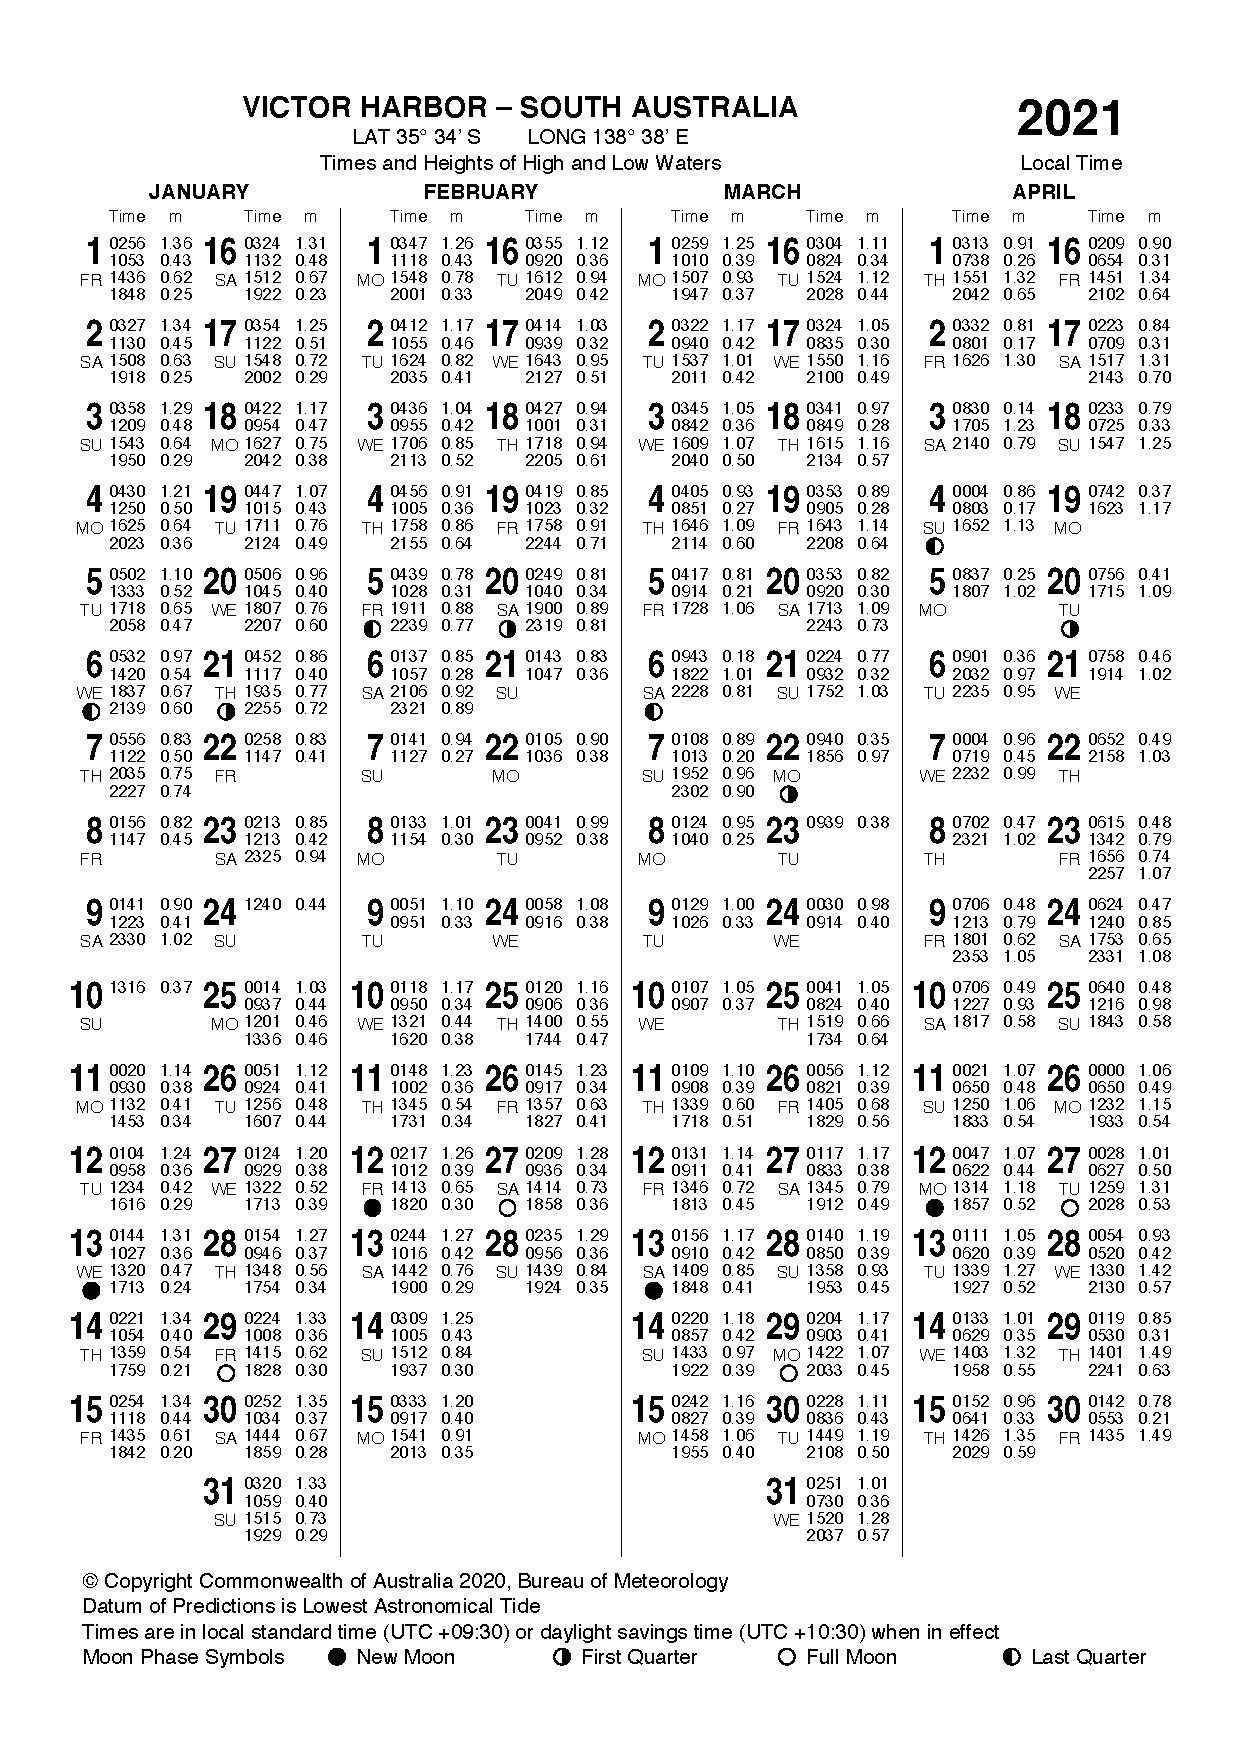
\includegraphics[trim={4cm 4cm 0 0 5cm},clip,width=0.4\textwidth]{figures/images/IDO59001_2021_SA_TP006.pdf}
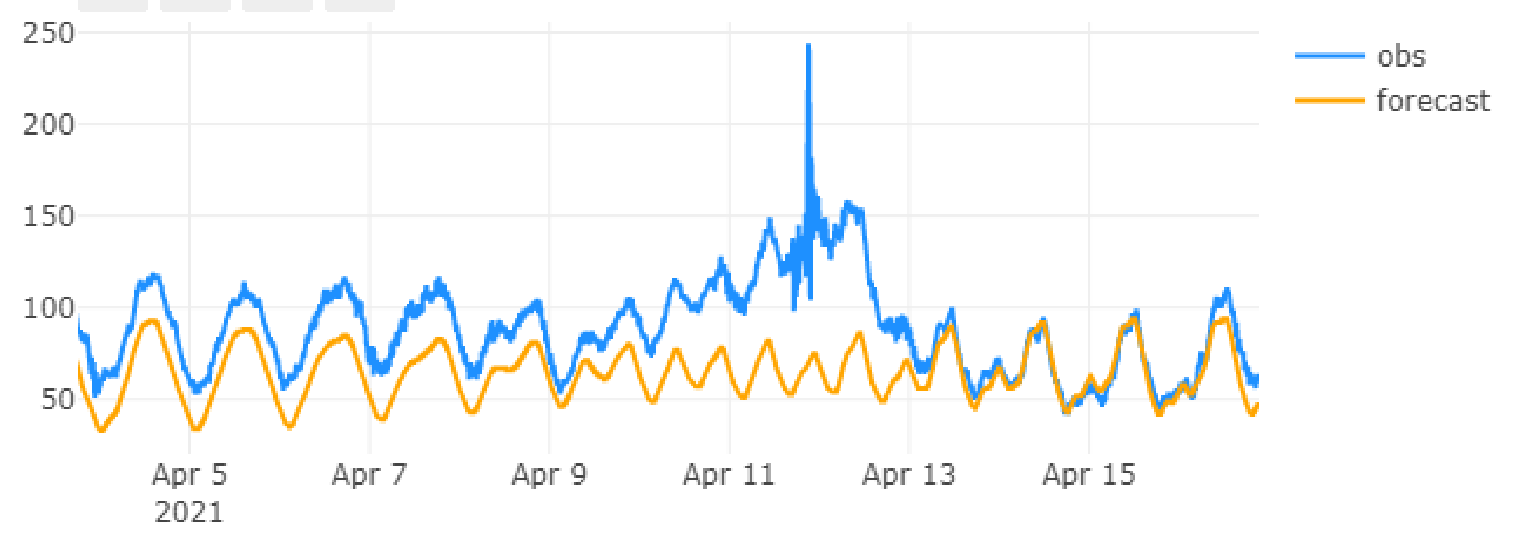
\includegraphics[height=0.3\textheight]{figures/plots/tide_eg_gero.png}
\hfill{}
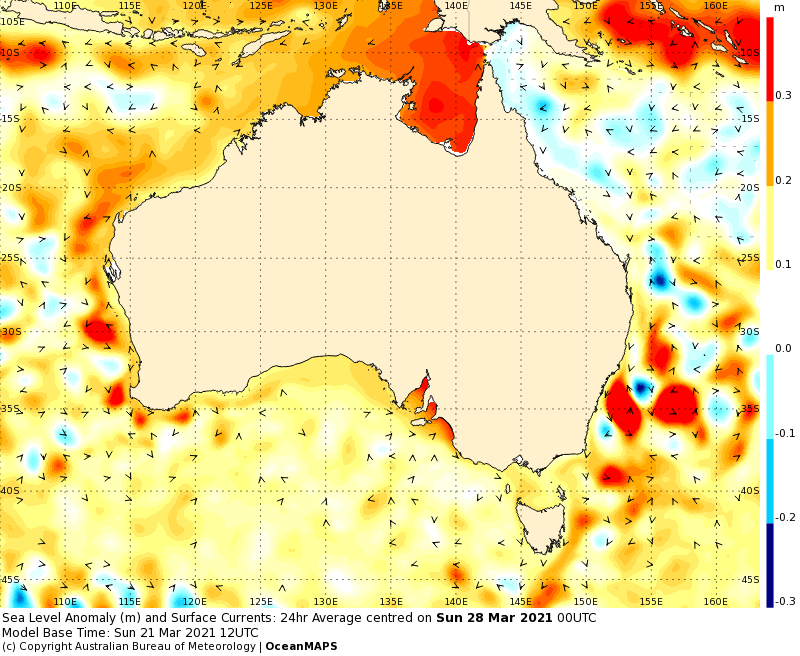
\includegraphics[height=0.3\textheight]{figures/images/IDYOC300.Aus.SLACur.168.png}
\end{frame}
%-----------------------------------------
\begin{frame}
\frametitle{Forecasts, physics, filters}
\centering
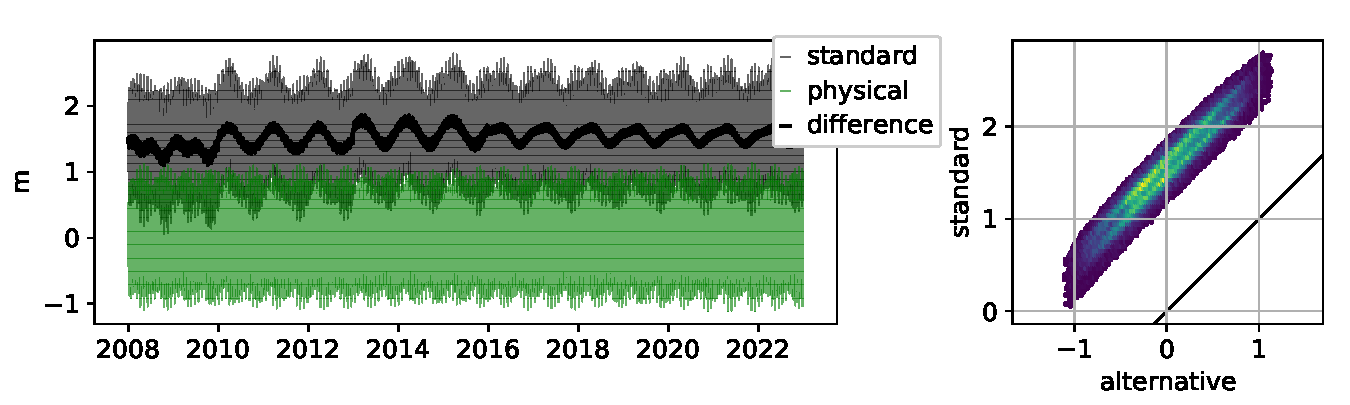
\includegraphics[width=\textwidth]{figures/plots/piecewiseTide_62430.pdf}
      \begin{itemize}
          \item standard annual tables are discontinuous
          \item poor choice for historical filter
          \item poor choice for physical attribution
          \item contrast purpose and context
      \end{itemize}
\end{frame}
%-----------------------------------------
\begin{frame}
\frametitle{Spatial models versus standard tides}
\begin{columns}
    \begin{column}{0.7\textwidth}      
    Different targets.\\
    Highlighted by mismatch at least "astronomical"\\
    Standard tides mixed quality too\\
    \hfill{}
    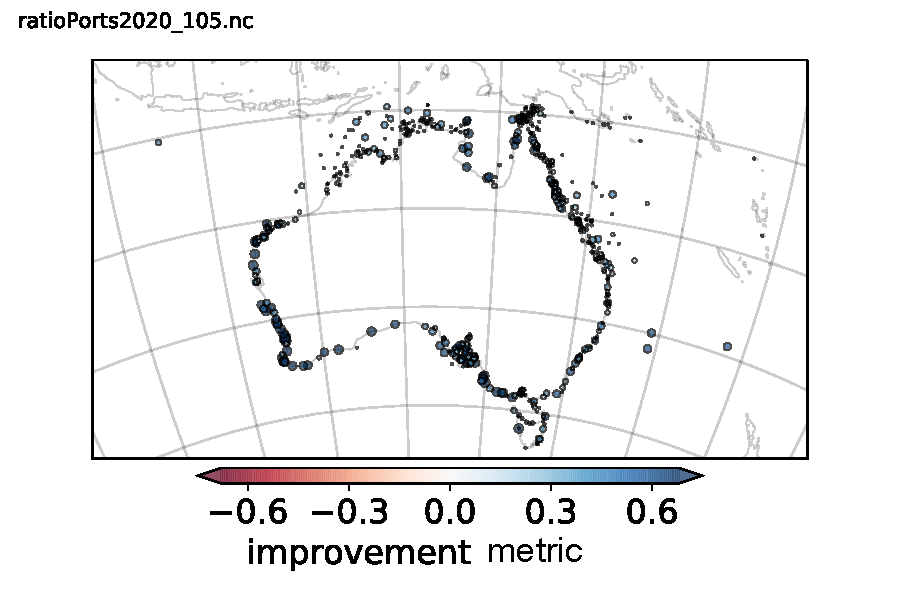
\includegraphics[width=\textwidth]{figures/maps/otpsPortCompare_Improve2020_105_diffRmse.pdf}
    \end{column}

    \begin{column}{0.3\textwidth}
      \begin{figure}      
        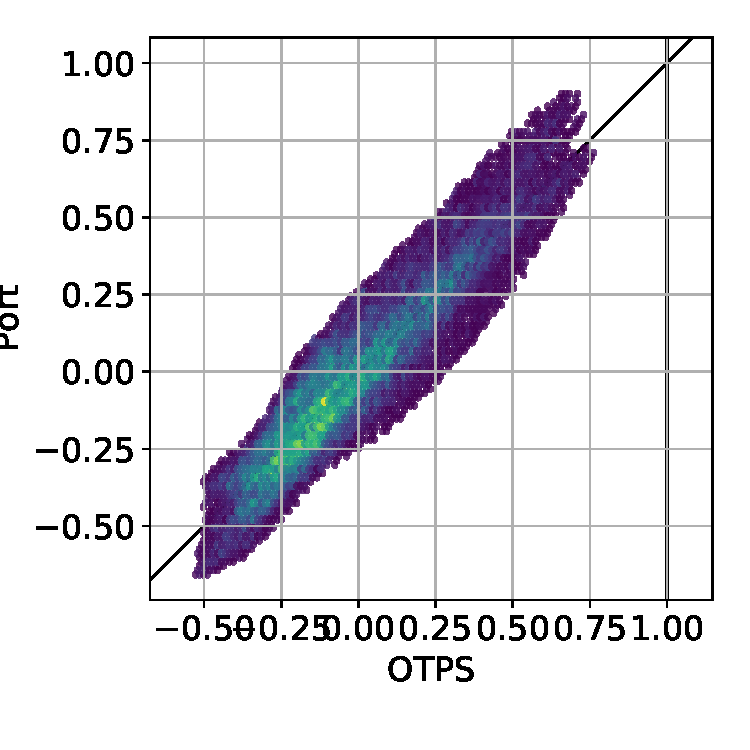
\includegraphics[height=0.25\textheight]{figures/plots/compareTides_61561_Full2020.pdf}
        \\
        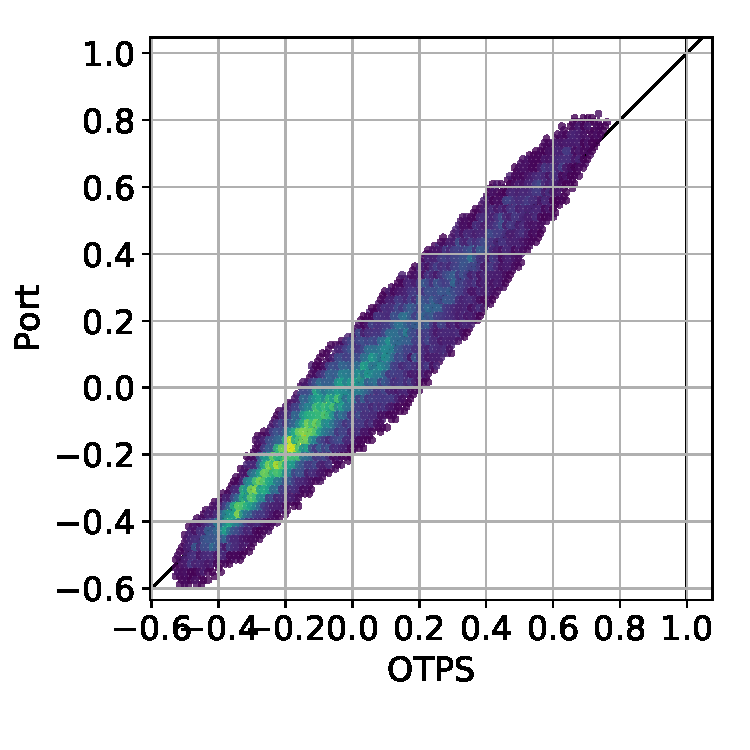
\includegraphics[height=0.25\textheight]{figures/plots/compareTides_61561_2020_201.pdf}
        \\
        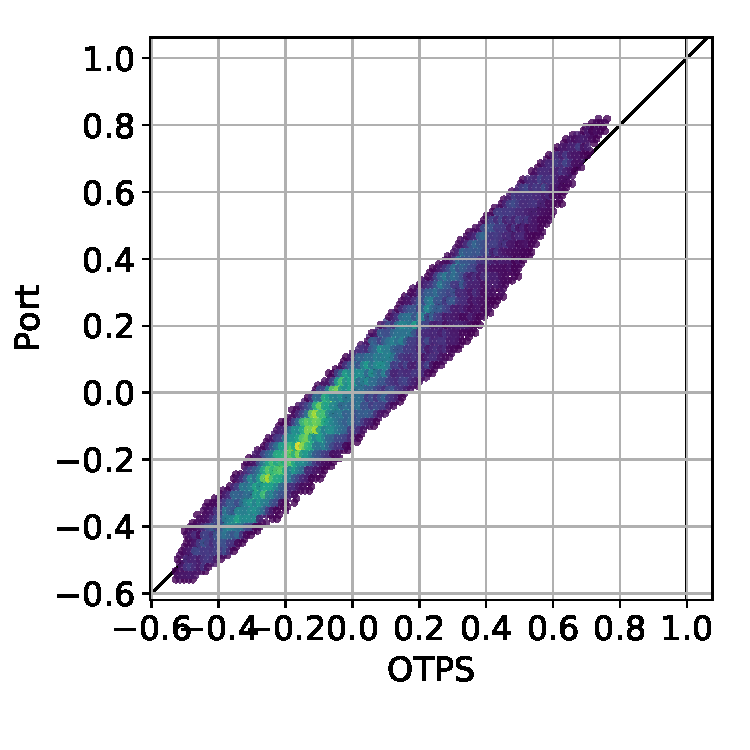
\includegraphics[height=0.25\textheight]{figures/plots/compareTides_61561_2020_105.pdf}
      \end{figure}
    \end{column}
\end{columns}
\end{frame}
%-----------------------------------------
\begin{frame}
\frametitle{Tidal service split}
Ongoing role for conventional service.\\
Clarify and differentiate targets to enable improvement. 
\vfill{}
    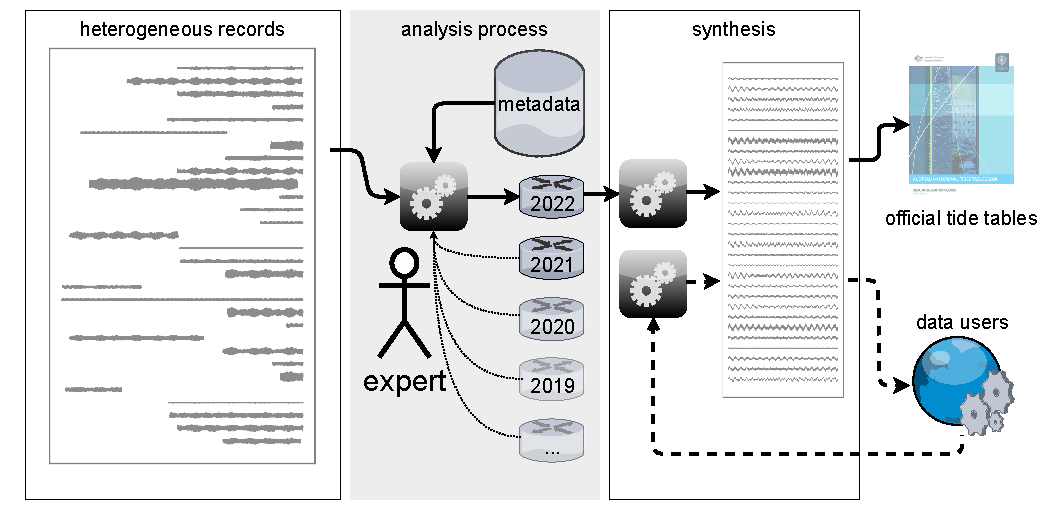
\includegraphics[height=0.6\textheight]{figures/diagrams/tideSchematic.pdf}
\end{frame}